% Sandia National Laboratories is a multimission laboratory managed and
% operated by National Technology & Engineering Solutions of Sandia, LLC, a
% wholly owned subsidiary of Honeywell International Inc., for the U.S.
% Department of Energy’s National Nuclear Security Administration under
% contract DE-NA0003525.

% Copyright 2002-2022 National Technology & Engineering Solutions of Sandia,
% LLC (NTESS).

% -------------------------------------------------------------------------
% Sampling Analysis Section ---------------------------------------------------
% -------------------------------------------------------------------------

\clearpage
\section{Polynomial Chaos Expansion (PCE) methods}
\label{PCE_Analysis}
\label{pce_Overview}
\index{analysis!PCE} \index{PCE analysis} 
\index{\texttt{.SAMPLING}}

\Xyce{} supports several styles of Polynomial Chaos expansion (PCE) methods, which are 
stochastic expansion methods that approximate the functional dependence
of a simulation response on uncertain model parameters by expansion
in a polynomial basis~\cite{XiuKarn02,Xiu2010}.   
In \Xyce{} the Stokhos library~\cite{stokhos} has been used to implement 
generalized PCE methods using the Wiener-Askey scheme\cite{XiuKarn02}.   

To propagate input uncertainty through a model using PCE, \Xyce{}
performs the following steps: (1) input uncertainties are transformed
to a set of uncorrelated random variables, (2) a basis such
as Hermite polynomials is selected, and (3) the parameters of the
functional approximation are determined.  The general PCE 
for a response $O$ has the form:
\begin{equation}
  O(p) \approx \hat{O}(p) = \sum_{i=0}^{P} \alpha^i \varPsi^i(p),
  \label{eq:genPCEresponse}
\end{equation}
where each multivariate basis polynomial $\varPsi^i(p)$ involves products of univariate
polynomials that are tailored to the individual random variables. 
More details about these methods and their \Xyce{} implementation can be found in
reference~\cite{xyceAdvancedUQ} and the references therein.

\Xyce{} supports three versions of polynomial chaos.  They mainly differ in how the coefficients $\alpha$ in equation~\ref{eq:genPCEresponse} are computed.  These three methods are:
\begin{itemize}
  \item Non-intrusive regression polynomial chaos (section~\ref{regressionPCE})
  \item Non-intrusive spectral projection  (NISP) (section~\ref{nisp})
  \item Fully intrusive spectral projection (section~\ref{intrusivePCE})
\end{itemize}
The first two versions are non-intrusive, meaning that they don't directly modify the forward problem being solved.  
Instead, they are augmentations to the \texttt{.SAMPLING} and \texttt{.EMBEDDEDSAMPLING} analysis methods.
The fully intrusive method is a separate analysis type, and is invoked using the \texttt{.PCE} command.
\clearpage
\subsection{Regression-based Polynomial Chaos}
\label{regressionPCE}

Regression-based PCE is briefly described in this section.
Regression-based PCE approaches aim to find the best fit for the linear system:
\begin{equation}
\boldsymbol{\varPsi} \boldsymbol{\alpha} \approx \boldsymbol{R} \label{eq:regression}
\end{equation}
for a set of PCE coefficients $\boldsymbol{\alpha}$ that best
reproduce a set of response values $\boldsymbol{R}$.   The orthogonal polynomials used in the  
PCE approximation are represented by the matrix $\varPsi$.  This matrix is usually a rectangular
matrix.

The regression approach finds a set of PCE coefficients $\alpha^i$ which best fit a set of response
values obtained from a sampling study on the density function of the uncertain 
parameters~\cite{pt_colloc1}.  One advantage of regression-based methods is that
they are very flexible with respect to the exact sample points used to evaluate the responses, 
and can readily be used with standard sampling methods such as Monte Carlo and Latin Hypercube Sampling.
The method that has been implemented in \Xyce{} for solving Eq.
\eqref{eq:regression} is least squares regression.

Regression-based PCE can be applied as a post-process step 
to \texttt{.SAMPLING} and \texttt{.EMBEDDEDSAMPLING}.  It is invoked by adding 
\texttt{regression\_pce=true} to the \texttt{.options SAMPLES} 
or \texttt{.options EMBEDDEDSAMPLES} command lines.  

Regression PCE will use the samples selected by the sampling algorithm (Monte Carlo or Latin Hypercube).  
The regression PCE algorithm will \emph{not} estimate the optimal number of samples to use, and so this must 
be set by the user.   For regression PCE, the number of samples needed for an accurate answer
can be smaller than the number that would have been required by conventional sampling.
For regression problems, to get an accurate answer it is considered good practice to oversample 
the basis size by at least a factor of 2. 

An example netlist, which uses regression PCE with \texttt{.SAMPLING} is given in figure~\ref{regressionPCE_Netlist1}.  
Results from this calculation, which are sent to terminal output are given in figure~\ref{regressionPCE_Result1}.
In this calculation, the polynomial order has been set to \texttt{5}, the output which is subject to the PCE analysis 
is \texttt{v(1)}, the type of sampling used is Latin Hypercube Sampling (LHS), and the results of the analysis are 
sent to terminal output.    For this example, the uncertain parameter is \texttt{testNorm}, which is
set by the \texttt{.param testNorm=\{aunif(2k,1k)\}} statement.  On the \texttt{.SAMPLING} line, 
the command \texttt{useExpr=true} instructs the sampling method to rely on expression-based 
random expressions.  Without this line, the sampling algorithm would ignore \texttt{testNorm}.

The parameter \texttt{resample=true} is a PCE-specific command.   Once the PCE approximation 
has been completed, the resulting polynomial can be thought of as a surrogate model, and this
surrogate can then be sampled, much like the original forward problem.  When the surrogate is 
sampled, it uses 1000 samples.    Since this calculation is sampling a polynomial, it can do 
a really large number of evaluations without incurring much computational expense.
The result of this resampling is (in the example) also sent to the console, as can be 
seen at the bottom of figure~\ref{regressionPCE_Result1}.

\begin{figure}[htbp]
\fontsize{9pt}{10pt}
\begin{centering}
\shadowbox{
\begin{minipage}{0.8\textwidth}
\begin{vquote}
\color{blue}Regression PCE example \color{black}
.param testNorm=\{\color{red}aunif(2k,1k)\color{black}\}
.param R1value=\{testNorm*2.0\}
R2 1 0 6K
R1 1 2 \{R1value\}
v1 2 0 1000V

.dc v1 1000 1000 1
.print dc format=tecplot v(1)
*
\color{red}.SAMPLING useExpr=true

.options SAMPLES numsamples=12
+ regression\_pce=true
+ order=5
+ outputs=\{v(1)\}
+ sample\_type=lhs
+ stdoutput=true
+ resample=true\color{black}
.end
\end{vquote}
\end{minipage}
}
\caption{Voltage divider regression PCE netlist.  The sampling-related commands are in \color{red}red\color{black}.
\label{regressionPCE_Netlist1}}
\end{centering}
\end{figure}

\begin{figure}[htbp]
\fontsize{9pt}{10pt}
\begin{centering}
\shadowbox{
\begin{minipage}{0.8\textwidth}
\begin{vquote}
***** Beginning Latin Hypercube Sampling simulation....

***** Regression PCE enabled.  Number of sample points = 12

***** PCE Basis size = 6

Seeding random number generator with 2412823737

LHS sampling mean of {V(1)} = 614.666
LHS sampling stddev of {V(1)} = 71.4563
LHS sampling variance of {V(1)} = 5106
LHS sampling skew of {V(1)} = 0.299928
LHS sampling kurtosis of {V(1)} = 2.07869
LHS sampling max of {V(1)} = 733.936
LHS sampling min of {V(1)} = 503.315

(traditional sampling) regression PCE mean of {V(1)} = 608.197
(traditional sampling) regression PCE stddev of {V(1)} = 71.3831

Statistics from re-sampling regression PCE approximation of {V(1)}:
mean     = 608.071
stddev   = 70.8532
variance = 5020.18
skew     = 0.298245
kurtosis = 1.93151
max      = 749.652
min      = 500.054
\end{vquote}
\end{minipage}
}
\caption{Voltage divider regression PCE result.  There are 3 sets of statistics in this ouptut.  
  The first set is computed from the 12 LHS sample points.  As this is a PCE calculation, the number of points is small and so the statistics based on them are probably not very accurate.
  The second set is computed from the PCE approximation, which are purely analytical.
  The third set is from running 1000 samples on the PCE approximation.  This output is enabled by \texttt{resample=true}.
\label{regressionPCE_Result1}}
\end{centering}
\end{figure}

\clearpage
\subsection{Non-Intrusive Spectral Projection (NISP)}
\label{nisp}
The spectral projection PCE approach projects the response
against each basis function $\Psi_j(p)$ using inner
products and employs the polynomial orthogonality properties to
extract each coefficient. Each inner product involves a
multidimensional integral over the support range of the weighting
function, which can be evaluated numerically using sampling,
tensor-product quadrature, Smolyak sparse grid \cite{Smolyak_63}, or
cubature \cite{stroud} approaches.   For the \Xyce{} implementation 
this means evaluating the following equation for each coefficient using 
quadrature rules:
\begin{equation}
\alpha^{i} = \frac{\langle O\varPsi ^{i}\rangle} {\langle (\varPsi ^{i})^{2}\rangle} = \frac{1} {\langle (\varPsi^{i})^{2}\rangle}\int _{\varGamma}O(p ;y)\varPsi ^{i}(y)\rho (y)dy = 0,\quad i = 0,\ldots,P.
  \label{nispProjection}
\end{equation}
In this equation $\rho$ is the joint density function, with respect to which the polynomials $\varPsi^i$ are orthogonal.
Evaluating this equation requires solving the integral on the right hand side.  
While many methods for solving this integral could be used, for the NISP algorithm 
the integral is solved using Gaussian Quadrature and related methods.  For this 
reason, these methods are sometimes referred to as ``quadrature PCE'' methods.
Stokhos supports several quadrature methods, and supplies the necessary quadrature points 
to \Xyce{} for the specified details.  

To solve the integral using quadrature, \Xyce{} has to evaluate the forward problem at 
the various quadrature points. In this reguard, this is similar to the
regression methods described in section~\ref{regressionPCE}, which has to do 
forward evaluations at randomly sampled points.
Since NISP uses quadrature points, the points are completely deterministic, 
and there are no random numbers involved.
The number of quadrature points can increase exponentially for larger numbers of uncertain 
parameters, but this can be mitigated by using sparse grid techniques.  

Non-intrusive spectral projection PCE can be applied as a post-process step 
to \texttt{.SAMPLING} and \texttt{.EMBEDDEDSAMPLING}.  It is invoked by adding 
\texttt{projection\_pce=true} to the \texttt{.options SAMPLES} 
or \texttt{.options EMBEDDEDSAMPLES} command lines.

As noted, when using NISP it is not necessary to specify the number of sample points, as they will
be set by the quadrature algorithm.  To enable quadrature on a sparse grid, set the 
option \texttt{sparse\_grid=true} on the \texttt{.options EMBEDDEDSAMPLES} command line.

An example netlist, which uses NISP with \texttt{.EMBEDDEDSAMPLING} is given in figure~\ref{NISP_netlist1}.  
Results from this calculation, which are output using the \texttt{.PRINT ES} command 
are given in figure~\ref{NISP_result1}.  The \texttt{.PRINT ES} command 
will automatically output several moments of the specified PCE outputs (in this 
case \texttt{V(drain)} and \texttt{V(gate)}) without any additional arguments 
on the \texttt{.PRINT ES} line.  In the example, additional information is 
requested using the \texttt{OUTPUT\_PCE\_COEFFS=TRUE} command, which will result 
in all of the PCE coefficients (the various $\alpha^{i}$ given by equation~\ref{nispProjection}).

A \texttt{.SAMPLING} version of the netlist given in figure~\ref{NISP_netlist1} can also be 
constructed, by simply replacing \texttt{.EMBEDDEDSAMPLING} with \texttt{.SAMPLING} and 
replacing \texttt{.options EMBEDDEDSAMPLES} with \texttt{.SAMPLES}.    However, the behavior
of \texttt{.SAMPLING} analysis will be a bit different.  As \texttt{.SAMPLING} 
performs the calculation for each quadrature point sequentially, rather than 
simultaneously, there is no equivalent of \texttt{.PRINT ES} for 
conventional sampling.  All of the \texttt{.SAMPLING} output is handled 
by the \texttt{.PRINT TRAN} command.  

Additionally, since the PCE analysis cannot be performed until the end of a 
\texttt{.SAMPLING} analysis, it is more  useful to have the analysis applied 
to \texttt{.MEASURE} commands which produce metrics for the entire simulation.  
Applying the PCE analysis to voltage node values in this case is less useful, 
as it will  simply use the final values for each voltage node (which will be 
mostly invariant in this example).

\begin{figure}[htbp]
\fontsize{9pt}{10pt}
\begin{centering}
\shadowbox{
\begin{minipage}{0.95\textwidth}
  \begin{vquote}\color{blue}
* embedded sampling with NISP, CMOS inverter\color{black}
.param inFreq=1e6, inPer=\{1/inFreq\}
.param td=\{inPer/2-inPer/10\}
.param tr=\{inPer/10\}, tf=\{inPer/10\}
.param pw=\{inPer/2-inPer/10\}, per=\{inPer\}

VS\_VDD vdd 0 DC 1.0
Vin gate 0 pulse( 0.0 1.0 \{td\} \{tr\} \{tf\} \{pw\} \{per\} )
M1 drain gate 0 0 NMOS w=0.18e-6 l=0.18e-6
M2 drain gate vdd vdd PMOS  w =0.54e-6 

.model nmos nmos (level=9 tnom=27 nch=2.3549e17 \color{red}vth0=\{aunif(0.55,0.15)\}\color{black} 
+ uc=5.105195e-11 ags=0.4044483 keta=-2.730673e-3 rdsw=105 wr=1 
+ dwg=-3.773529e-9 dwb=5.239518e-9 cit=0 cdscb=0 dsub=0.0167866 
+ pdiblc2=3.38377e-3 pscbe1=8e10 delta=0.01 prt=0 kt1l=0 ub1=-7.61e-18 
+ wl=0 wwn=1 lln=1 lwl=0 cgdo=7.9e-10 cj=9.539798e-4 
+ cjsw=2.53972e-10 cjswg=3.3e-10 cf=0 pk2=-4.42044e-4 pu0=10.8203648 
+ pvsat=1.388017e3 tox=4.1e-9 k2=1.63871e-3 w0=1e-7 dvt1w=0 
+ dvt1=0.3683763 ua=-1.504141e-9 vsat=9.896282e4 b0=-4.706134e-8 
+ a1=5.916677e-4 prwg=0.5 wint=0 voff=-0.0883818 cdsc=2.4e-4 
+ eta0=2.470369e-3 pclm=0.7326932 pdiblcb=-0.1 pscbe2=1.254966e-9 
+ rsh=6.5 ute=-1.5 kt2=0.022 uc1=-5.6e-11 wln=1 wwl=0 lw=0 
+ capmod=2 cgso=7.9e-10 pb=0.8 pbsw=0.8 pbswg=0.8 pvth0=7.505753e-4 
+ wketa=3.100384e-3 pua=2.896652e-11 peta0=8.758549e-5 toxm=4.1e-9 
+ xj=1e-7 k1=0.6064385 k3b=2.763267 dvt0w=0 dvt0=1.3330881 u0=258.9066683 
+ nlx=1.71872e-7 dvt2w=0 dvt2=0.0540199 ub=2.428646e-18 a0=1.8904342 
+ k3=1e-3 b1=1.294942e-6 a2=0.9069159 prwb=-0.2 lint=1.69494e-8 
+ nfactor=2.1821266 cdscd=0 etab=1.047744e-5 pdiblc1=0.1823102 
+ drout=0.7469045 pvag=0 mobmod=1 kt1=-0.11 ua1=4.31e-9 at=3.3e4 
+ ww=0 ll=0 lwn=1 xpart=0.5 cgbo=1e-12 mj=0.380768 mjsw=0.1061193 
+ mjswg=0.1061193 prdsw=-2.7650517 lketa=-0.0104103 
+ pub=1.684125e-23 pketa=1.549791e-3)

.model pmos pmos (level=9 tnom=27 nch=4.1589e17 \color{red}vth0=\{-aunif(0.55,0.15)\}\color{black} 
+ k2=0.0258663 w0=1e-6 dvt1w=0 dvt0=0.6117215 u0=106.5280265 uc=-1e-10 
+ ags=0.3667554 keta=0.0237092 rdsw=304.9893888 wr=1 dwg=-2.44019e-8 
+ dwb=-9.06003e-10 cit=0 cdscb=0 dsub=1.0998181 pdiblc2=0.0420477 
+ pscbe1=1.073111e10 delta=0.01 prt=0 kt1l=0 ub1=-7.61e-18 
+ wl=0 wwn=1 lln=1 lwl=0 cgdo=6.41e-10 cj=1.200422e-3 
+ cjsw=2.001802e-10 cjswg=4.22e-10 cf=0 pk2=1.799383e-3 pu0=-1.3399122 
+ pvsat=-50 l=0.18e-6 tox=4.1e-9 k3=0 nlx=1.20187e-7 
+ dvt2w=0 dvt1=0.2286816 ua=1.125454e-9 vsat=1.593712e5 b0=5.263128e-7 
+ a1=0.2276342 prwg=0.5 wint=0 voff=-0.0878287 cdsc=2.4e-4 eta0=0.1672562 
+ pclm=2.2249148 pdiblcb=-1e-3 pscbe2=3.099395e-9 rsh=7.4 ute=-1.5 
+ kt2=0.022 uc1=-5.6e-11 wln=1 wwl=0 lw=0 capmod=2 cgso=6.41e-10 
+ pb=0.8478616 pbsw=0.8483594 pbswg=0.8483594 pvth0=2.098588e-3 
+ wketa=0.0295614 pua=-5.27759e-11 peta0=1.003159e-4 toxm=4.1e-9 
+ xj=1e-7 k1=0.59111 k3b=7.9143108 dvt0w=0 dvt2=0.1 ub=1e-21 a0=1.6904754 
+ b1=1.496707e-6 a2=0.6915706 prwb=0.2553725 lint=3.217673e-8 
+ nfactor=1.8560303 cdscd=0 etab=-0.1249603 pdiblc1=8.275696e-4 
+ drout=0 pvag=15 mobmod=1 kt1=-0.11 ua1=4.31e-9 at=3.3e4 ww=0 ll=0 
+ lwn=1 xpart=0.5 cgbo=1e-12 mj=0.4105254 mjsw=0.3400571 
+ mjswg=0.3400571 prdsw=4.4771801 lketa=-1.935751e-3 
+ pub=1e-21 pketa=-3.434535e-3)

\color{red}.EMBEDDEDSAMPLING useExpr=true
.options EMBEDDEDSAMPLES outputs=\{v(drain)\},\{V(gate)\} projection\_pce=true
.PRINT ES OUTPUT\_PCE\_COEFFS=TRUE FORMAT=tecplot \color{black}
.tran 1ns 0.75e-6
.PRINT TRAN v(drain) V(gate)
.END
\end{vquote}
\end{minipage}
}
\caption{CMOS Inverter Non-intrusive Spectral Projection (NISP) netlist. 
 The NISP-related commands are in \color{red}red\color{black}.
\label{NISP_netlist1}}
\end{centering}
\end{figure}

\begin{figure}[hbt]
\centering
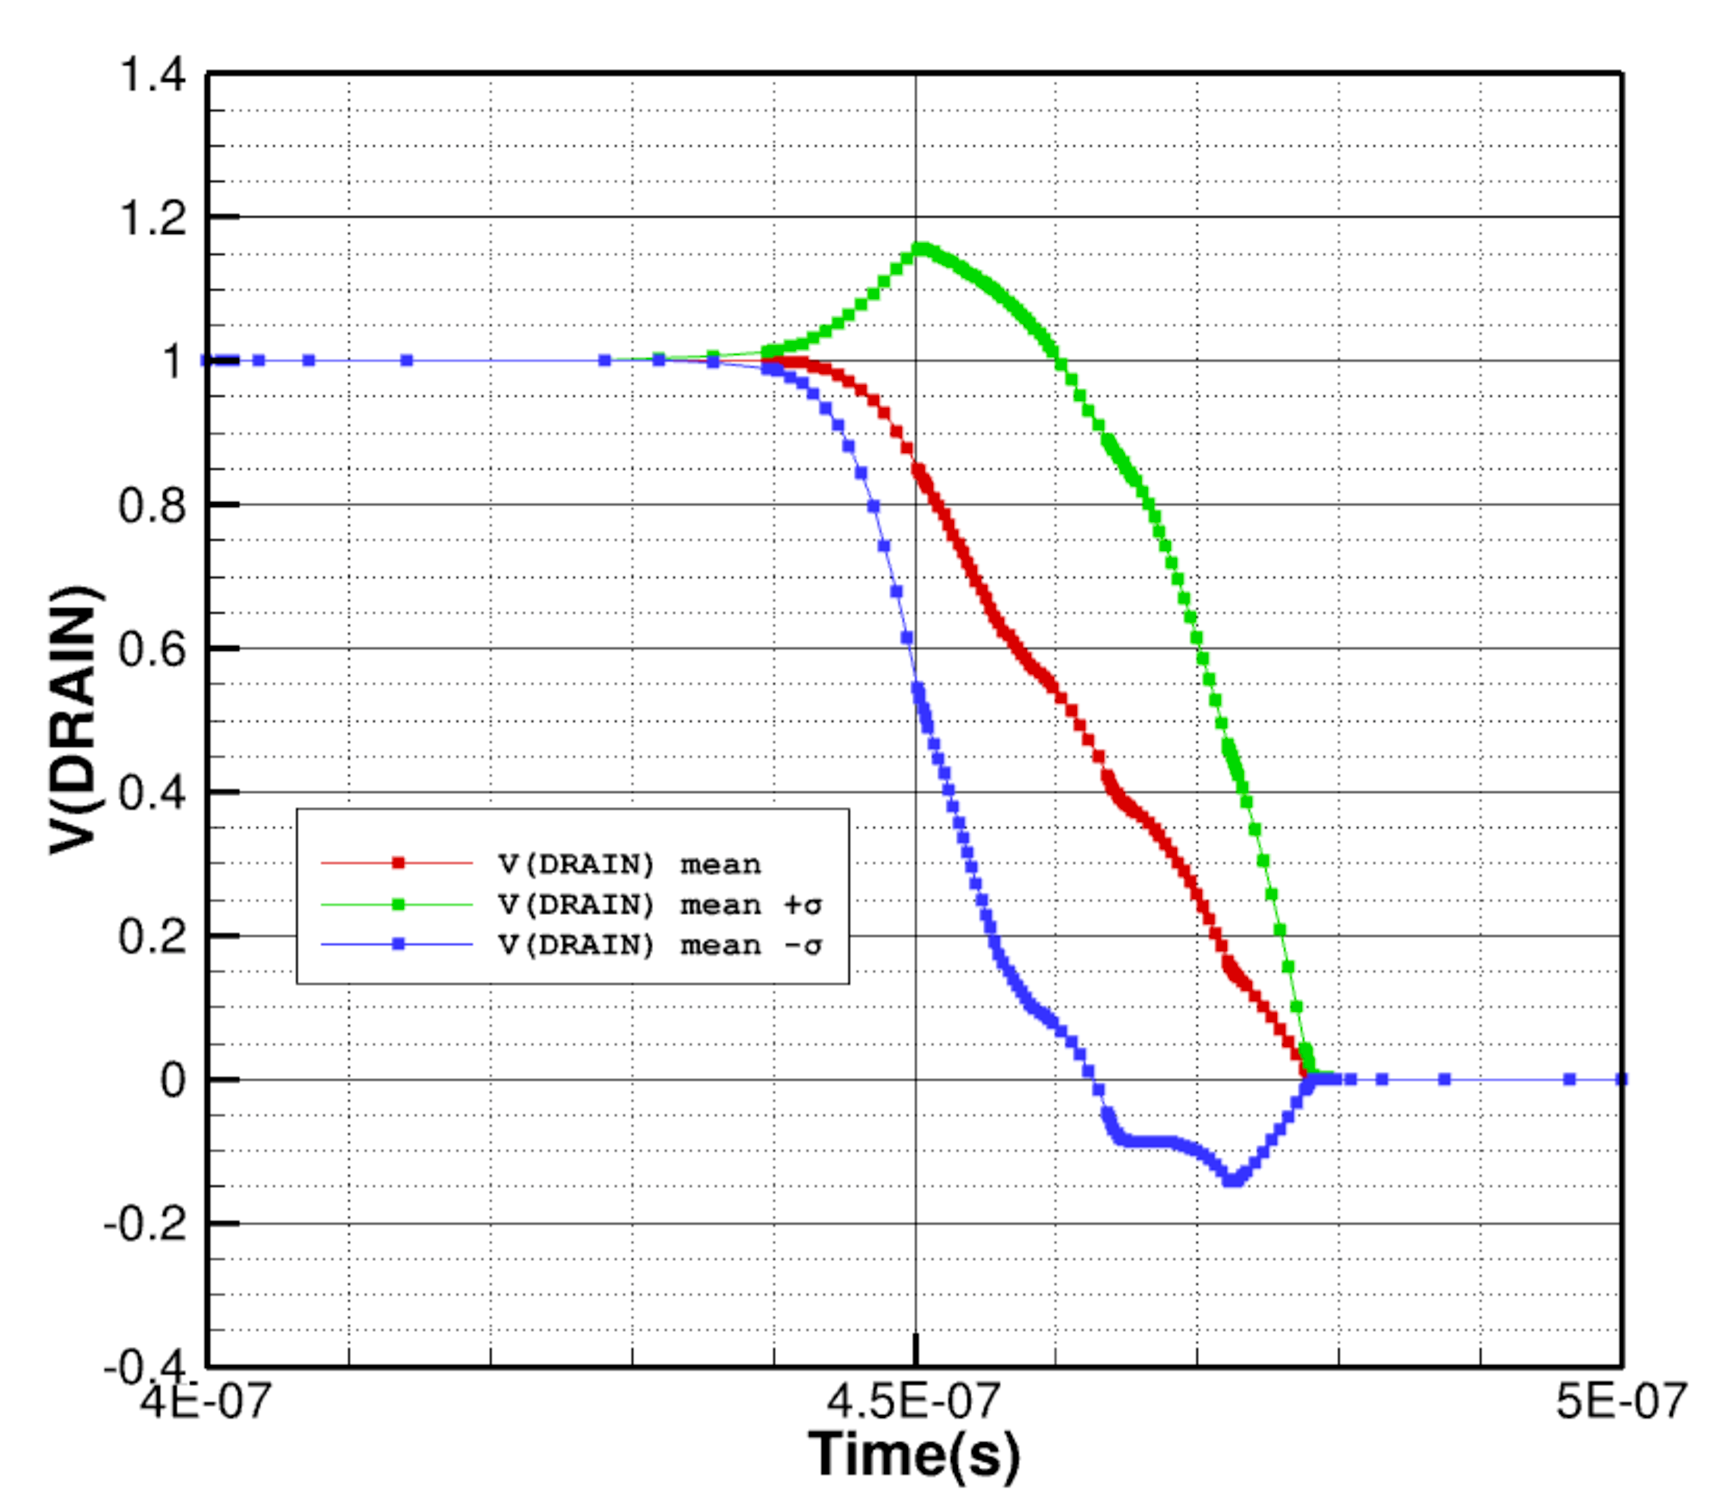
\includegraphics[width=5in]{cmos_inverter_result.pdf}
\caption
  [CMOS Inverter NISP Output] {CMOS Inverter NISP Output}
\label{NISP_result1}
\end{figure}

\clearpage
\subsection{Fully Intrusive Spectral Projection}
\label{intrusivePCE}
The fully intrusive form of PCE involves solving a system of equations which is constructed by 
applying the orthogonal polynomial expansion defined by 
Eq. \eqref{eq:genPCEresponse} to all the terms of the differential-algebraic 
system of equations solved by \Xyce{}.  The details of this construction are given in 
reference~\cite{xyceAdvancedUQ}.  This method is primarily experimental at this
point, and is inherently more expensive,
so it is not the best choice of PCE method in \Xyce{}.   Most \texttt{.PCE} use cases of
interest can be computed much more cheaply and robustly using \texttt{.EMBEDDEDSAMPLING} 
combined with one of the non-intrusive PCE methods (regression PCE or NISP).
Similar to \texttt{.EMBEDDEDSAMPLING} based calculations, \texttt{.PCE} computes
PCE coefficients at every stage of the calculation.   

An example netlist, for a diode clipper circuit which uses intrusive PCE, is given in figure~\ref{Fully_Intrusive_PCE_netlist1}.
For this type of analysis, it is not necessary to specify \texttt{projection\_pce=true}.  The result for this circuit 
is given in figure~\ref{Fully_Intrusive_PCE_result1}.  
\begin{figure}[htbp]
\fontsize{9pt}{10pt}
\begin{centering}
\shadowbox{
\begin{minipage}{0.95\textwidth}
  \begin{vquote}\color{blue}Transient Diode Clipper with intrusive PCE analysis\color{black}

.tran 2ns 2.0ms

\color{red}.PCE useExpr=true
.options PCES 
+ OUTPUTS=R4:R,D1N3940:IS outputs=\{V(4)\}
.print pce format=tecplot \color{black}

VCC 1 0 5V
VIN 3 0 SIN(0V 10V 1kHz)
D1 2 1 D1N3940
D2 0 2 D1N3940
R1 2 3 1K
R2 1 2 3.3K
R3 2 0 3.3K
R4 4 0 \color{red} \{aunif(9.0k,6.0k)\} \color{black}
C1 2 4 0.47u

.MODEL D1N3940 D(
+ \color{red} IS=\{aunif(4.0e-10,2.0e-10)\} \color{black}
+ RS=.105 N=1.48 TT=8E-7
+ CJO=1.95E-11 VJ=.4 M=.38 EG=1.36
+ XTI=-8 KF=0 AF=1 FC=.9 BV=600 IBV=1E-4)
.END 
\end{vquote}
\end{minipage}
}
\caption{Diode clipper fully intrusive PCE netlist.
 The PCE-related commands are in \color{red}red\color{black}.
\label{Fully_Intrusive_PCE_netlist1}}
\end{centering}
\end{figure}

\begin{figure}[hbt]
\centering
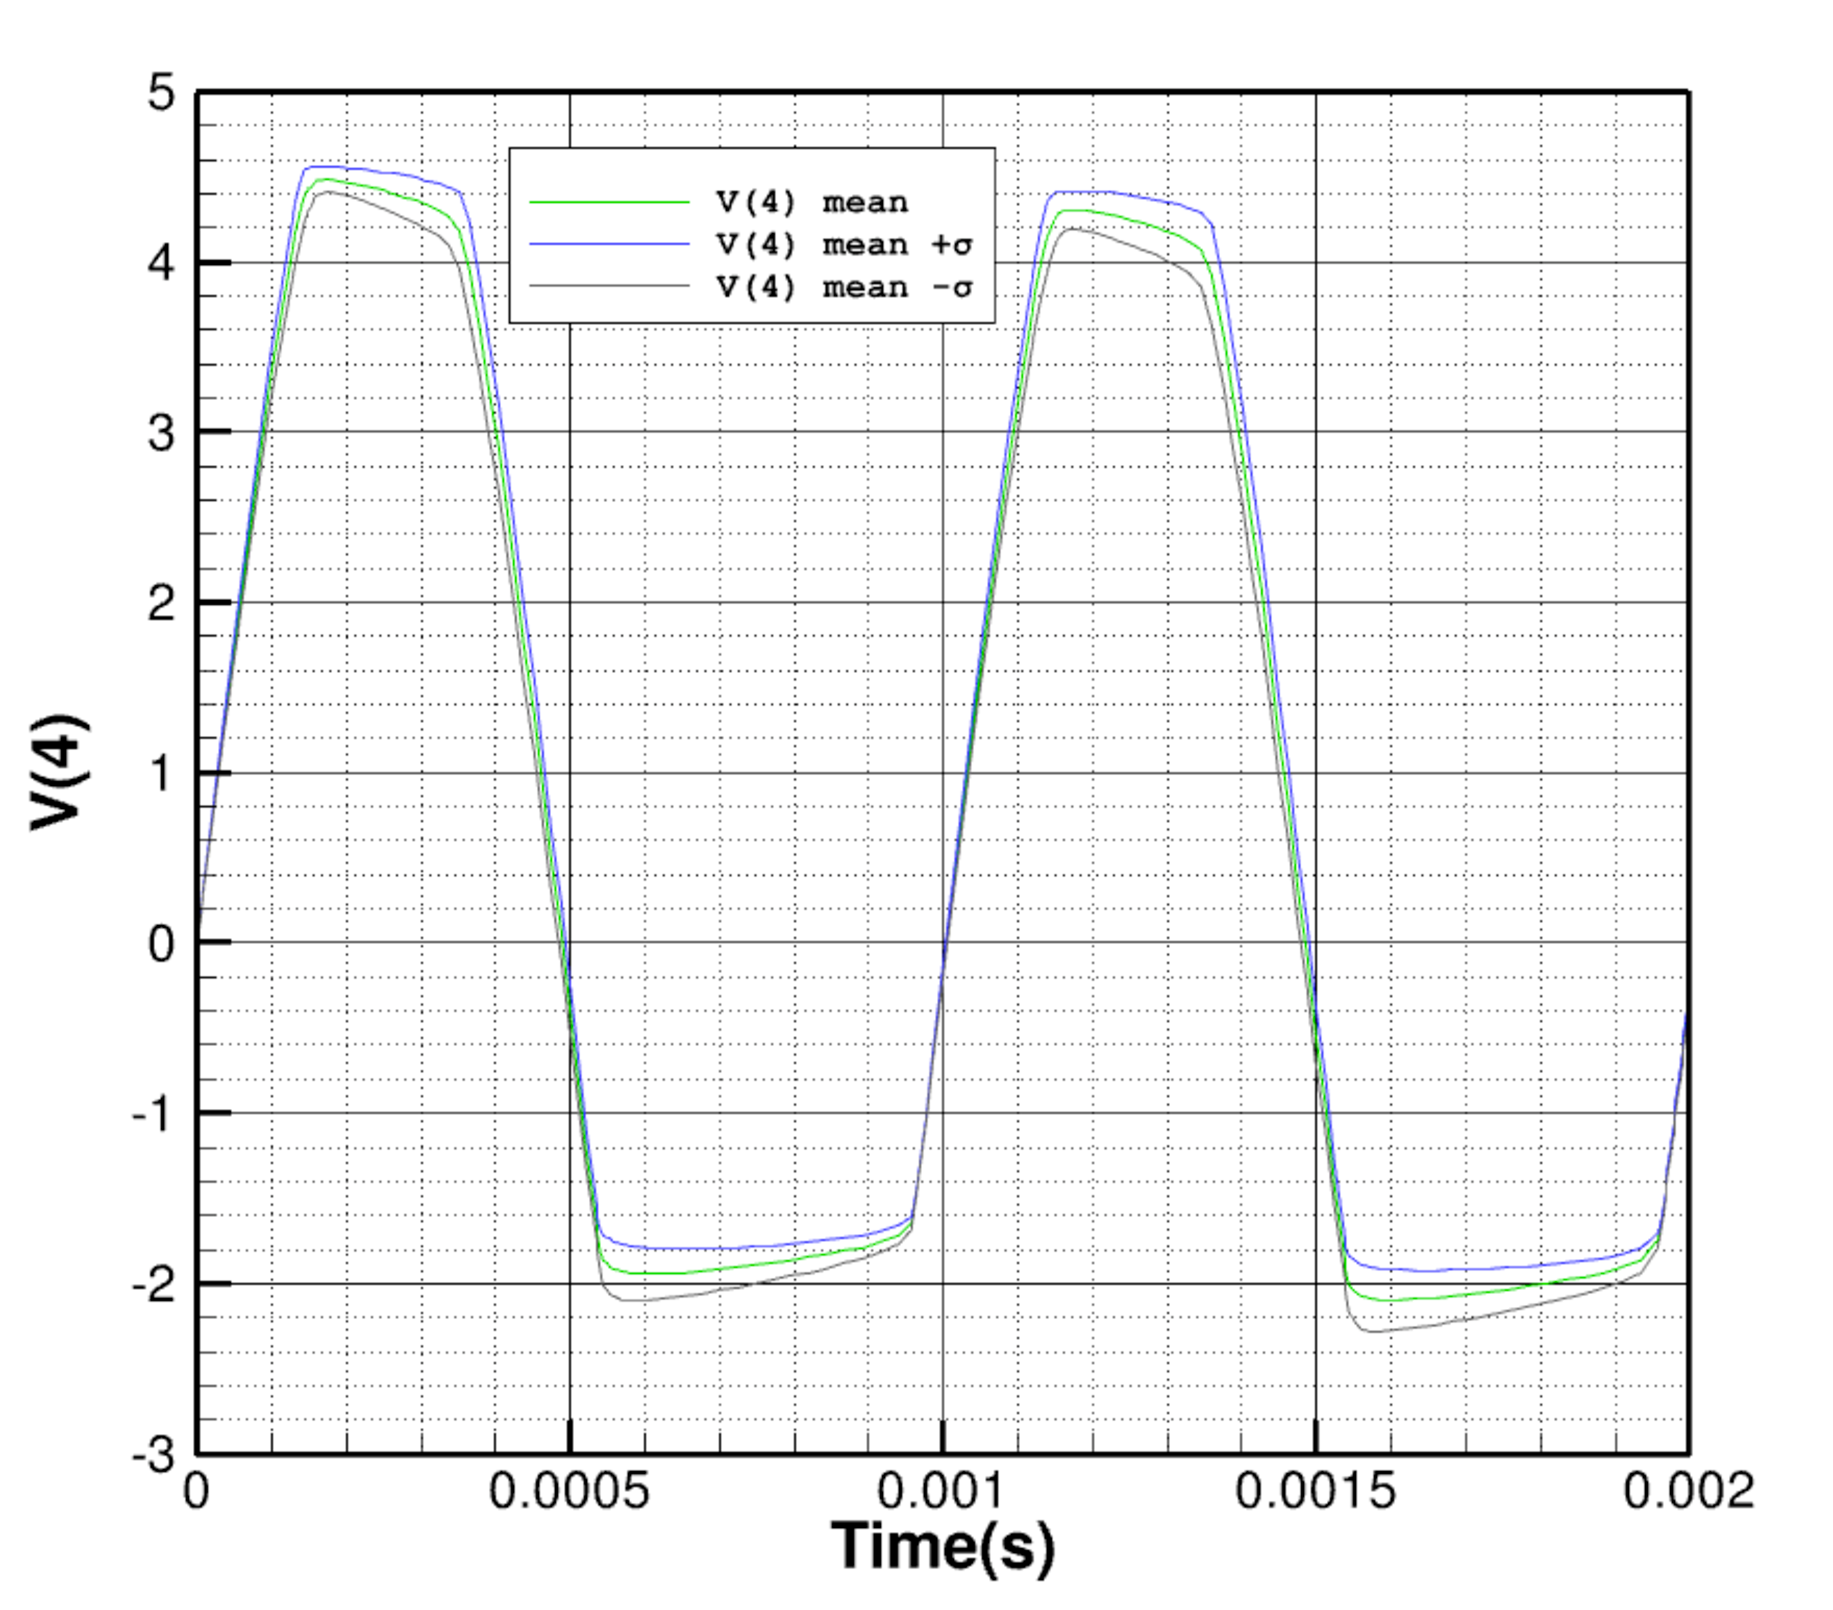
\includegraphics[width=5in]{clipperPce2.pdf}
\caption
  [Diode clipper fully intrusive PCE Output] {Diode clipper fully intrusive PCE Output}
\label{Fully_Intrusive_PCE_result1}
\end{figure}

\clearpage
%% -----------------------------------------------------------------------------------
\subsection{Comparing PCE methods: Gilbert Cell Mixer PCE example}
\label{xyceGilbertCell}
A Gilbert cell mixer circuit is given in figure~\ref{gilbert}~\cite{1049925}.  A corresponding netlist 
is given in Fig.~\ref{NISP_gilbert_netlist}.
In this circuit, the LO voltage is given by \texttt{v(6,2)} and \texttt{v(15,10)} is the input. 
The output is the difference between collector voltages of Q4/Q6 and Q3/Q5 (\texttt{V(5,3)}), 
and should be the approximate product of the LO and input voltages.
In this example, all eight resistors are given uncertain resistances,
distributed with the following normal distributions:  R1 and R2 are N(10,1), R5
and R6 are N(100,5), and R3, R4, R7, and R8 are N(1500,50).  These large
standard deviations of the resistances are not realistic, but are chosen for
demonstration purposes.
\begin{figure}[hbt]
\centering
\resizebox{.9\linewidth}{!}{ \input cktFigs/gilbert}
  \caption[Gilbert cell mixer schematic]
  {Gilbert cell mixer schematic.}
\label{gilbert}
\end{figure}

Ensemble and PCE results for the Gilbert cell mixer are shown in figure~\ref{gilbert_compare}.   
As this calculation was concerned with the transient behavior, only \texttt{.EMBEDDEDSAMPLING} 
and \texttt{.PCE} are used in this example.  For \texttt{.EMBEDDEDSAMPLING}, both types of 
non-intrusive PCE are used.
The light grey lines in Fig.~\ref{gilbert_compare} are for all the sample points 
of an embedded LHS study with 1000 samples.    The red lines (which are obscured 
by other results) show the mean and the mean +/- twice the standard deviation for the 
1000 sample study.  This can be considered the ``gold'' standard for this simulation.
The other solid lines show the moments from the various PCE calculations, and they 
lie on top of the 1000 LHS sample moments.  

This version of the netlistgiven in Fig.~\ref{NISP_gilbert_netlist}
is using non-intrusive projection PCE as an augmentation to \texttt{.EMBEDDEDSAMPLING}.  
To convert this netlist to 
use the fully intrusive method, change \texttt{.EMBEDDEDSAMPLING} to \texttt{.PCE}, and 
change \texttt{.options EMBEDDEDSAMPLES} to \texttt{.options PCES}.   Otherwise, the commands are completely the same.
As the number of uncertain parameters is a little bit larger (8), for the projection-based methods a 
Smolyak sparse grid~\cite{Smolyak_63} method is used.  This is set with the  \texttt{sparse\_grid=true} parameter. 
Using the sparse grid, the number of 
required quadrature points for this problem is 129.  Using the non-sparse Gaussian quadrature 
would have required 6561 quadrature points. This would have rendered the method much 
less efficient than sampling, and basically not usable, especially for the \texttt{.PCE} method.

To change the netlist to use non-intrusive regression PCE, change \texttt{projection\_pce=true} 
to \texttt{regression\_pce=true}.  Delete the \texttt{sparse\_grid=true} parameter, as 
it isn't relevant to regression PCE.  

As noted, for regression PCE the number of parameters needs to be set.  Unlike projection-based methods, 
regression PCE does not have a rigid requirement for the number of samples.  For this 
problem the size of the polynomial basis is 45, and for regression problems it 
is considered good practice to oversample by at least a factor of 2, which implies that
a good choice for this circuit is 90 sample points.   
To set this, add \texttt{numsamples=90} on the \texttt{.options EMBEDDEDSAMPLES} line.  
It appears that 90 sampling points was 
adequate for the regression form of PCE, as the all the statistical moments 
match well throughout the transient.

\begin{figure}[htbp]
\fontsize{10pt}{11pt}
\begin{centering}
\shadowbox{
\begin{minipage}{0.95\textwidth}
  \begin{vquote}\color{blue}
* Gilbert cell mixer\color{black}
R5 1 2 \color{red}\{agauss(100,5,1)\}\color{black}
Q3 3 2 4 QB2T2222
Q4 5 6 4 QB2T2222
Q5 3 6 8 QB2T2222
Q6 5 2 8 QB2T2222
R6 2 1 \color{red}\{agauss(100,5,1)\}\color{black}
*the local oscillator
VLO 6 2 DC 0 SIN(0 .05V 4e7 0 0)
Q1 4 10 11 QB2T2222
R1 11 12 \color{red}\{agauss(10,1,1)\}\color{black}
R2 12 13 \color{red}\{agauss(10,1,1)\}\color{black}
* input bias current
I1 12 0 DC 1.8mA
Q2 8 15 13 QB2T2222
R4 15 16 \color{red}\{agauss(1500,50,1)\}\color{black}
R3 16 10 \color{red}\{agauss(1500,50,1)\}\color{black}
V1 16 0 DC 1.8V
*the input voltage to be mixed with the LO
V5 15 10 DC 0 sin(0 .05V 3e6 0 0)
R7 5 17 \color{red}\{agauss(1500,50,1)\}\color{black}
R8 3 17 \color{red}\{agauss(1500,50,1)\}\color{black}
V3 17 0 DC 8V
V2 1 0 DC 6V

.MODEL QB2T2222  NPN (
+ IS=3.136905E-14 BF=189 NF=0.9977664 VAF=29.7280913
+ IKF=0.7405619 ISE=8.49314E-15 NE=1.3186316 BR=38.9531224
+ NR=0.9833179 VAR=28.5119855 IKR=4.632395E-3 ISC=4.624043E-14
+ NC=1.225899 RB=2.0158781 IRB=0.0227681 RBM=0.9730261
+ RE=0.0501513 RC=0.6333 CJE=2.369655E-11 VJE=0.6884357
+ MJE=0.3054743 TF=5.3E-10 XTF=48.5321578 VTF=5.3020062
+ ITF=1.1 PTF=14.6099207 CJC=8.602583E-12 VJC=0.4708887
+ MJC=0.3063885 XCJC=1 TR=74E-9 CJS=1e-12 VJS=.75
+ MJS=0 XTB=0.87435 EG=1.11 XTI=5.825
+ KF=0 AF=1 FC=0.5)

.TRAN 1ns 3e-7
.PRINT TRAN format=tecplot v(6,2) v(15,10) v(5,3)
.options timeint reltol=1.0e-5 
    \color{red}
.EMBEDDEDSAMPLING useExpr=true
.options EMBEDDEDSAMPLES projection\_pce=true 
+ outputs={v(5,3)} order=2 sparse\_grid=true \color{black}
.end
\color{blue}\end{vquote}
\end{minipage}
}
\caption{Gilbert Cell Non-Instrusive Spectral Project (NISP) netlist.  
  UQ commands are in \color{red}red\color{black}, and NISP is specified using the \texttt{projection\_pce} parameter.
\label{NISP_gilbert_netlist}}
\end{centering}
\end{figure}

NISP is used in conjunction with embedded sampling, 
and as noted requires 129 sample points if using sparse grid quadrature.  Fully 
intrusive PCE, which uses all the same machinery as NISP also requires 129 
quadrature points.  



\begin{figure}[hbt]
\centering
\includegraphics[width=5in]{gilbert_compare2.pdf}
\caption
  [Gilbert Cell Mixer Output for several \Xyce{} embedded UQ methods]
  {Gilbert Cell Mixer Output for several \Xyce{} embedded UQ methods.  The mean and standard deviations for all the methods (Embedded LHS sampling, NISP, Regression PCE and fully intrusive PCE) all match very well.}
\label{gilbert_compare}
\end{figure}

\clearpage
